\documentclass{article}
\usepackage{amsfonts} 
\usepackage{amsmath}
\usepackage{hyperref}
\usepackage{graphicx}
\usepackage{subcaption}
\usepackage{booktabs}
\usepackage{makecell}
\usepackage{multirow}
%\usepackage{placeins}

\begin{document}

\section{Description}
\par The first we just calculated several Barycentric Cubical Tori. The distribution of calculated toruses we can see in the Figure \ref{fig:cases_distribution}.
\begin{figure}[htbp]
    \centering
    \begin{subfigure}[t]{0.45\textwidth}
        \centering
        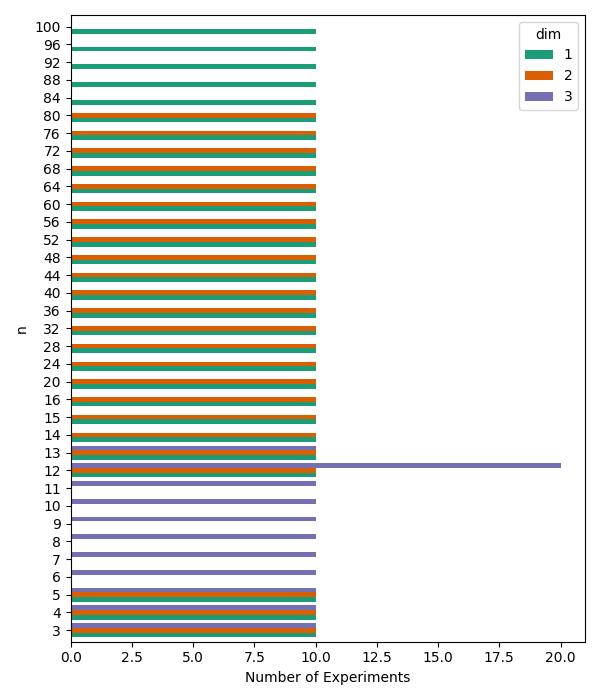
\includegraphics[width=\textwidth]{pics/torus scores/cases.png}
        \caption{Barycentric Cubical Tori}
        \label{fig:cases_distribution}
    \end{subfigure}
    \hfill
    \begin{subfigure}[t]{0.45\textwidth}
        \centering
        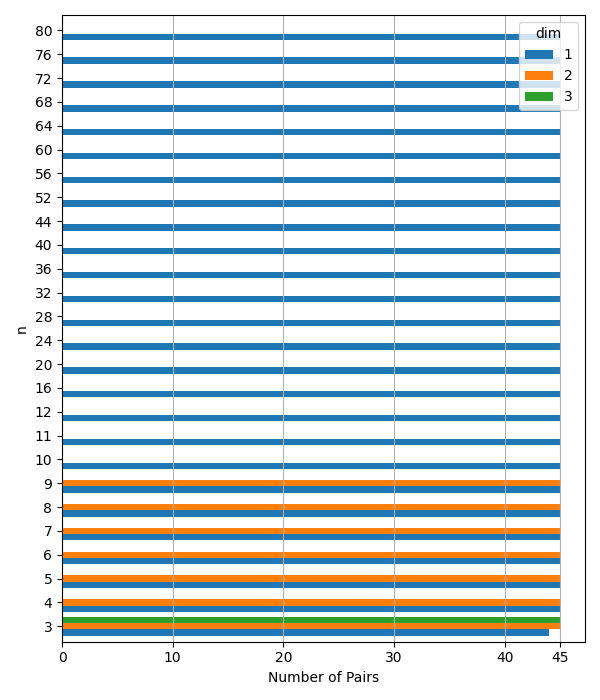
\includegraphics[width=\textwidth]{pics/torus-transpositions/distribution.png}
        \caption{Calculated pairs}
        \label{fig:pairs_distribution}
    \end{subfigure}
    \caption{Size/dimension distribution}
    \label{fig:distribution}
\end{figure}

\par Then for each pair of filtrations with similar dimension and $n$ $f_0, f_1:\mathbb{T}^d_n \to \mathbb{R}$ we can define a linear homotopy $h: [0, 1]\times\mathbb{T}^d_n \to \mathbb{R}$:
$$
    h(t, \sigma) = (1 - t)\cdot f_0(\sigma) + t\cdot f_1(\sigma)
$$

\par The moment of time $t\in [0, 1]$ such there exist a pair of cells $\sigma_0, \sigma_1\in\mathbb{T}^d_n$ such that $h(t, \sigma_0) = h(t, \sigma_1)$ is a moment of transposition of these cells during the homotopy (the probability, that this will be full segment is 0 for pair of independent barycentric cubical tori).
\par We have found all transposing pairs like this, classified them and calculated how these transpositions cahnges the Depth Poset. The distribution of calculated pairs of filtration we can see in the Figure \ref{fig:pairs_distribution}.

\section{Transpositions}
\par There could be 3 types of cell in the terms of birth-death pairs:
\begin{itemize}
    \item \textbf{Births} - The cells which are births of some cycles
    \item \textbf{Deaths} - The cells which are deaths of some cycles
    \item \textbf{Unpaired} - The cells which are not birth or deaths of any cycle
\end{itemize}

\par So we have defined 5 types of transpositions:
\begin{itemize}
    \item \textbf{Birth-Birth} - The switch transpositions of 2 brith cells
    \item \textbf{Birth-Death} - The switch transpositions of brith and death cells
    \item \textbf{Death-Death} - The switch transpositions of 2 death cells
    \item \textbf{Undefined} - The transpositions where at least 1 cell is unpaired
    \item \textbf{No switch} - No switch transposition, where all cells are paired
\end{itemize}

\par In the Figure \ref{fig:switch-full} we can see the mean count of transpositions of each type for barycentric cubical tori of different dimensions $d$ and size $n$.
We can see that no switch transpositions are majority of cases. So we also can look at Figure \ref{fig:switch-without-noswitch} to get how other types are distributed.

\begin{figure}[h!]
    \hspace*{-3cm}
    \centering
    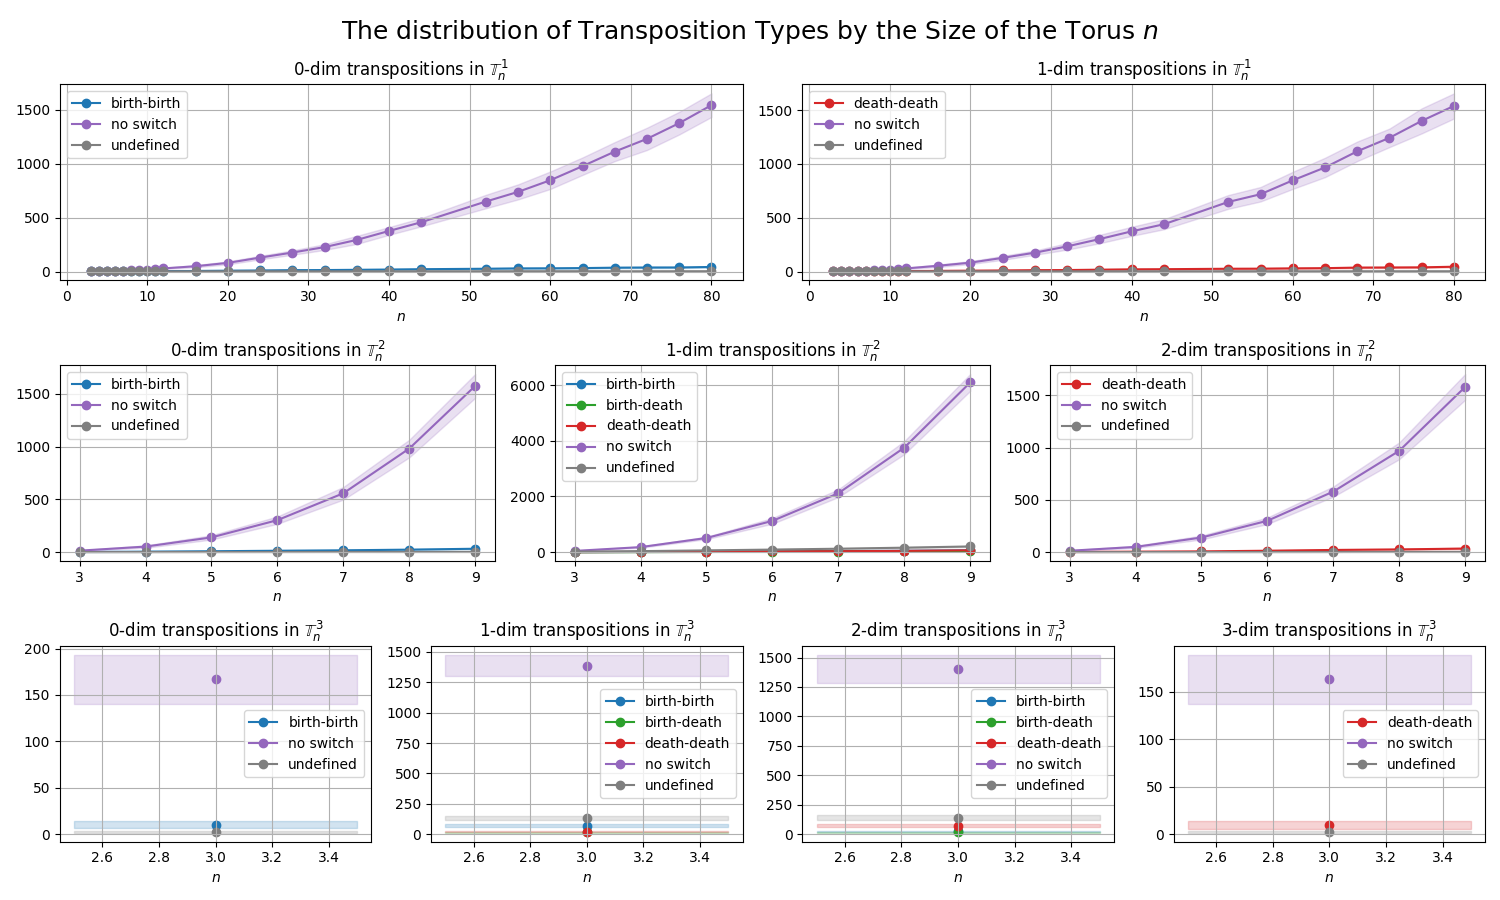
\includegraphics[width=1.5\textwidth]{pics/torus-transpositions/switch-types.png}
    \caption{The mean value of number of transpositions of each type.}
    \label{fig:switch-full}
\end{figure}

\begin{figure}[h!]
    \hspace*{-3cm}
    \centering
    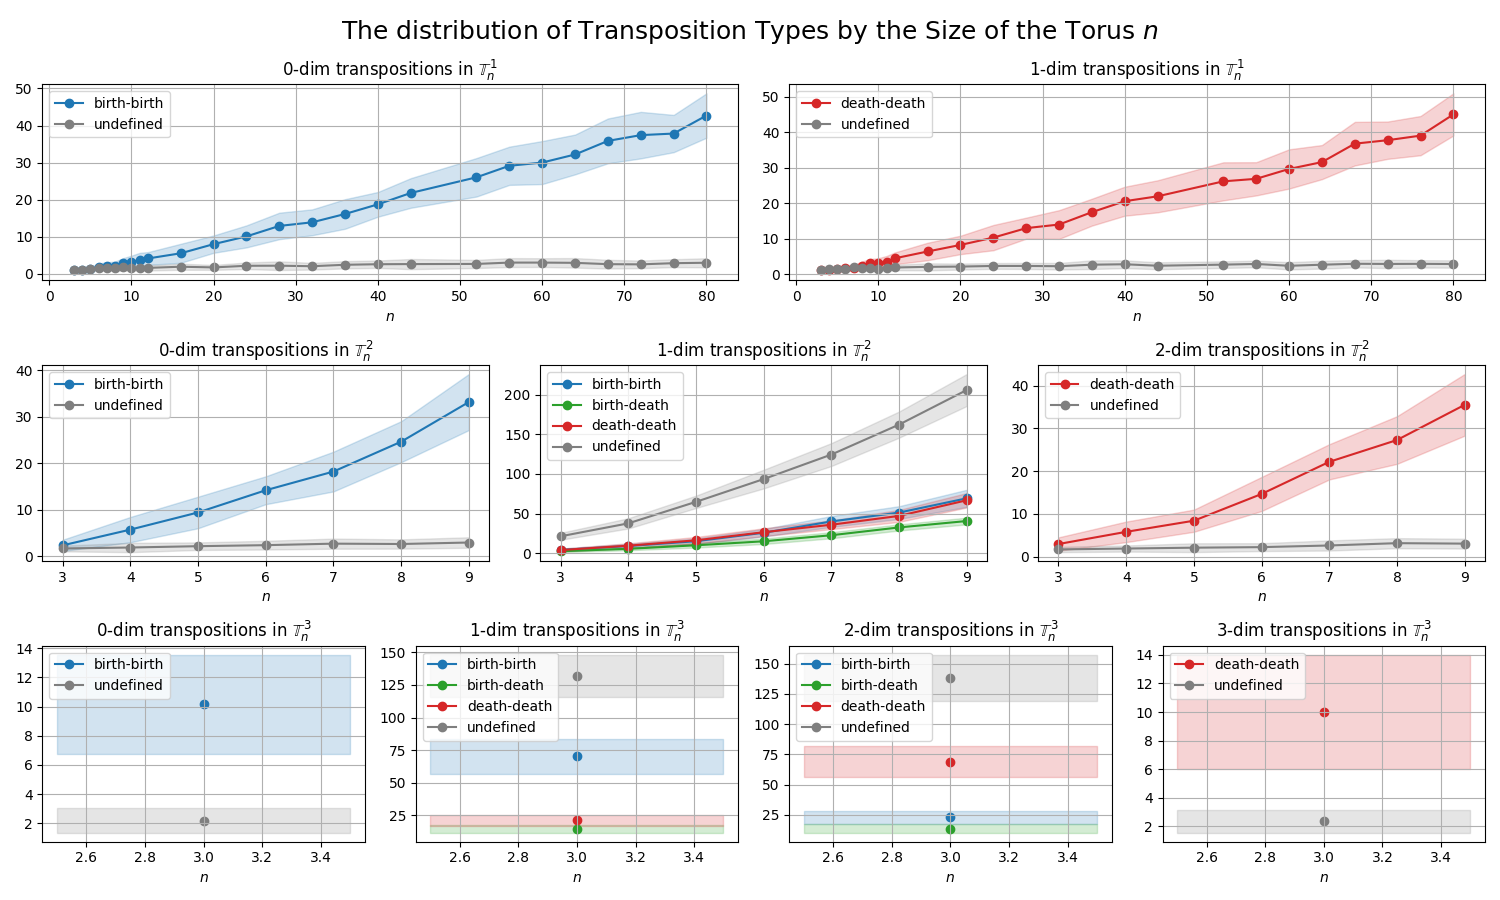
\includegraphics[width=1.5\textwidth]{pics/torus-transpositions/switch-types (without no switch).png}
    \caption{The mean value of number of transpositions of each type (without no switch transpositions).}
    \label{fig:switch-without-noswitch}
\end{figure}



\section{Similarity Scores}

\par We have 10 scores to measure the similarity of 2 depth posets: 
\begin{itemize}
\item \textbf{birth\_relation\_cell\_similarity} - The Jacard index of arcs (edges) in the birth relation (given by row left to right reduction algorithm).
    Consider 2 birth-death pairs are similar if they corespond the similar cells.
We can see the values of this score applying to depth posets before and after transpositions of different types for barycentric cubical tori dimension $d$ and size $n$ in Figure \ref{fig:birth-relation-cell-similarity}
\item \textbf{birth\_relation\_index\_similarity} - The Jacard index of arcs (edges) in the birth relation (given by row left to right reduction algorithm).
    Consider 2 birth-death pairs are similar if ther indices in the filtration pairs are similar.
We can see the values of this score applying to depth posets before and after transpositions of different types for barycentric cubical tori dimension $d$ and size $n$ in Figure \ref{fig:birth-relation-index-similarity}
\item \textbf{death\_relation\_cell\_similarity} - The Jacard index of arcs (edges) in the death relation (given by column bottom to top reduction algorithm).
    Consider 2 birth-death pairs are similar if they corespond the similar cells.
We can see the values of this score applying to depth posets before and after transpositions of different types for barycentric cubical tori dimension $d$ and size $n$ in Figure \ref{fig:death-relation-cell-similarity}
\item \textbf{death\_relation\_index\_similarity} - The Jacard index of arcs (edges) in the death relation (given by column bottom to top reduction algorithm).
    Consider 2 birth-death pairs are similar if ther indices in the filtration pairs are similar.
We can see the values of this score applying to depth posets before and after transpositions of different types for barycentric cubical tori dimension $d$ and size $n$ in Figure \ref{fig:death-relation-index-similarity}
\item \textbf{poset\_arc\_cell\_similarity} - The Jacard index of arcs (edges) in the Depth Poset.
    Consider 2 birth-death pairs are similar if they corespond the similar cells.
We can see the values of this score applying to depth posets before and after transpositions of different types for barycentric cubical tori dimension $d$ and size $n$ in Figure \ref{fig:poset-arc-cell-similarity}
\item \textbf{poset\_arc\_index\_similarity} - The Jacard index of arcs (edges) in the Depth Poset.
    Consider 2 birth-death pairs are similar if ther indices in the filtration pairs are similar.
We can see the values of this score applying to depth posets before and after transpositions of different types for barycentric cubical tori dimension $d$ and size $n$ in Figure \ref{fig:poset-arc-index-similarity}
\item \textbf{poset\_node\_cell\_similarity} - The Jacard index of nodes (elements) in the Depth Poset.
    Consider 2 birth-death pairs are similar if they corespond the similar cells.
We can see the values of this score applying to depth posets before and after transpositions of different types for barycentric cubical tori dimension $d$ and size $n$ in Figure \ref{fig:poset-node-cell-similarity}
\item \textbf{poset\_node\_index\_similarity} - The Jacard index of nodes (elements) in the Depth Poset.
    Consider 2 birth-death pairs are similar if ther indices in the filtration pairs are similar.
We can see the values of this score applying to depth posets before and after transpositions of different types for barycentric cubical tori dimension $d$ and size $n$ in Figure \ref{fig:poset-node-index-similarity}
\item \textbf{relation\_cell\_similarity} - The Jacard index of arcs (edges) in the relation (given by reduction algorithms).
    Consider 2 birth-death pairs are similar if they corespond the similar cells.
We can see the values of this score applying to depth posets before and after transpositions of different types for barycentric cubical tori dimension $d$ and size $n$ in Figure \ref{fig:relation-cell-similarity}
\item \textbf{relation\_index\_similarity} - The Jacard index of arcs (edges) in the relation (given by reduction algorithms).
    Consider 2 birth-death pairs are similar if ther indices in the filtration pairs are similar.
We can see the values of this score applying to depth posets before and after transpositions of different types for barycentric cubical tori dimension $d$ and size $n$ in Figure \ref{fig:relation-index-similarity}
\end{itemize}
%\par We used these scores to measure the similarity of depth poset before and after the transpositions, and we can see the result in coresponding Figures.
\begin{figure}[h!]
    \hspace*{-3cm}
    \centering
    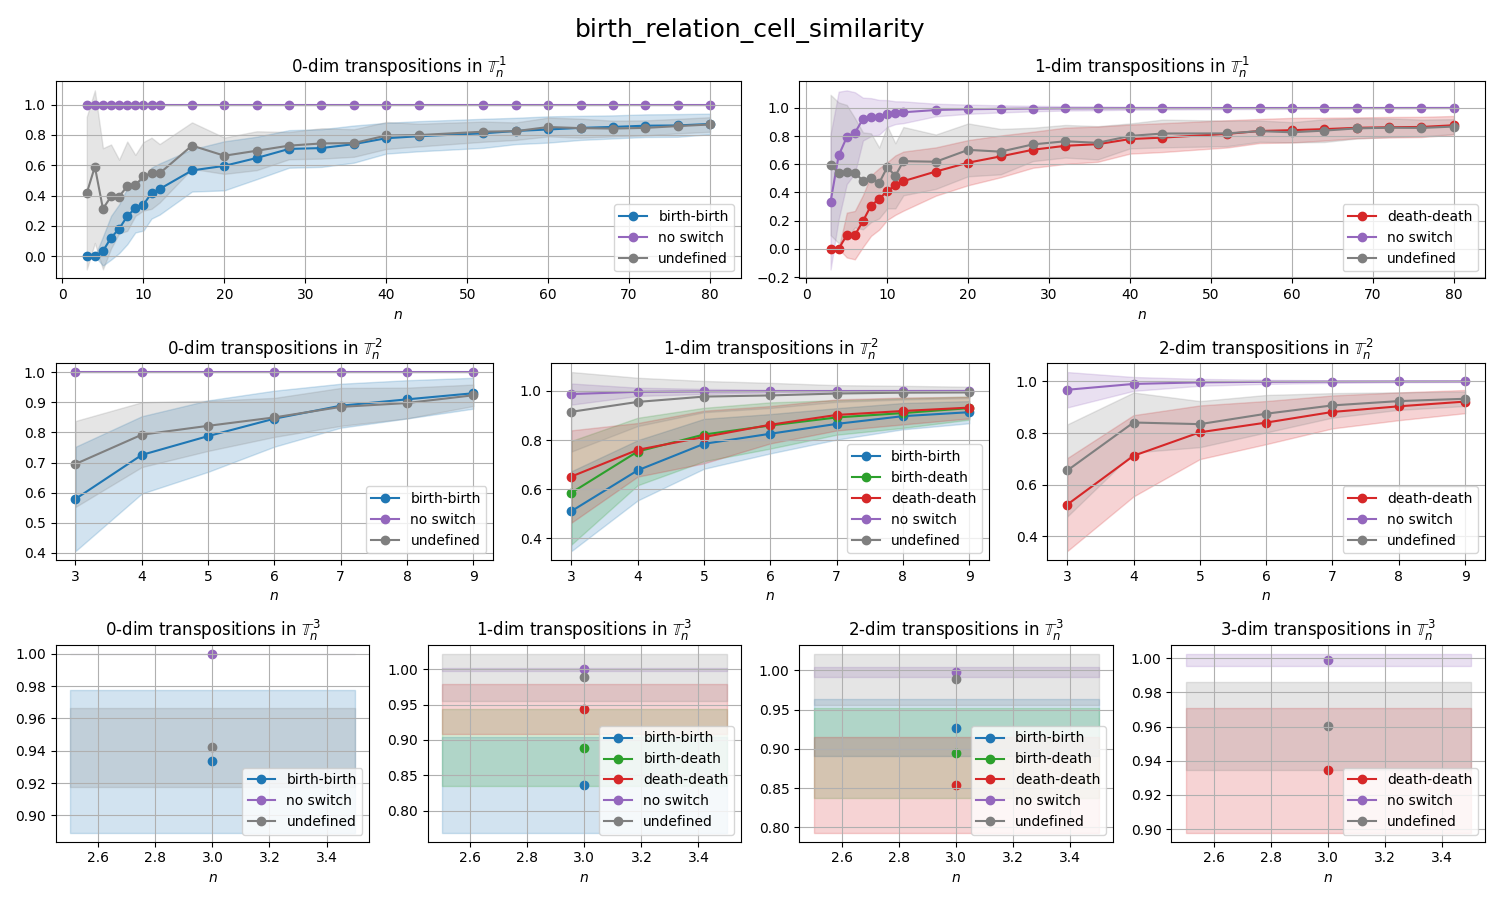
\includegraphics[width=1.5\textwidth]{pics/torus-transpositions/similaritites/score=birth-relation-cell-similarity.png}
    \caption{birth\_relation\_cell\_similarity values}
    \label{fig:birth-relation-cell-similarity}
\end{figure}
\begin{figure}[h!]
    \hspace*{-3cm}
    \centering
    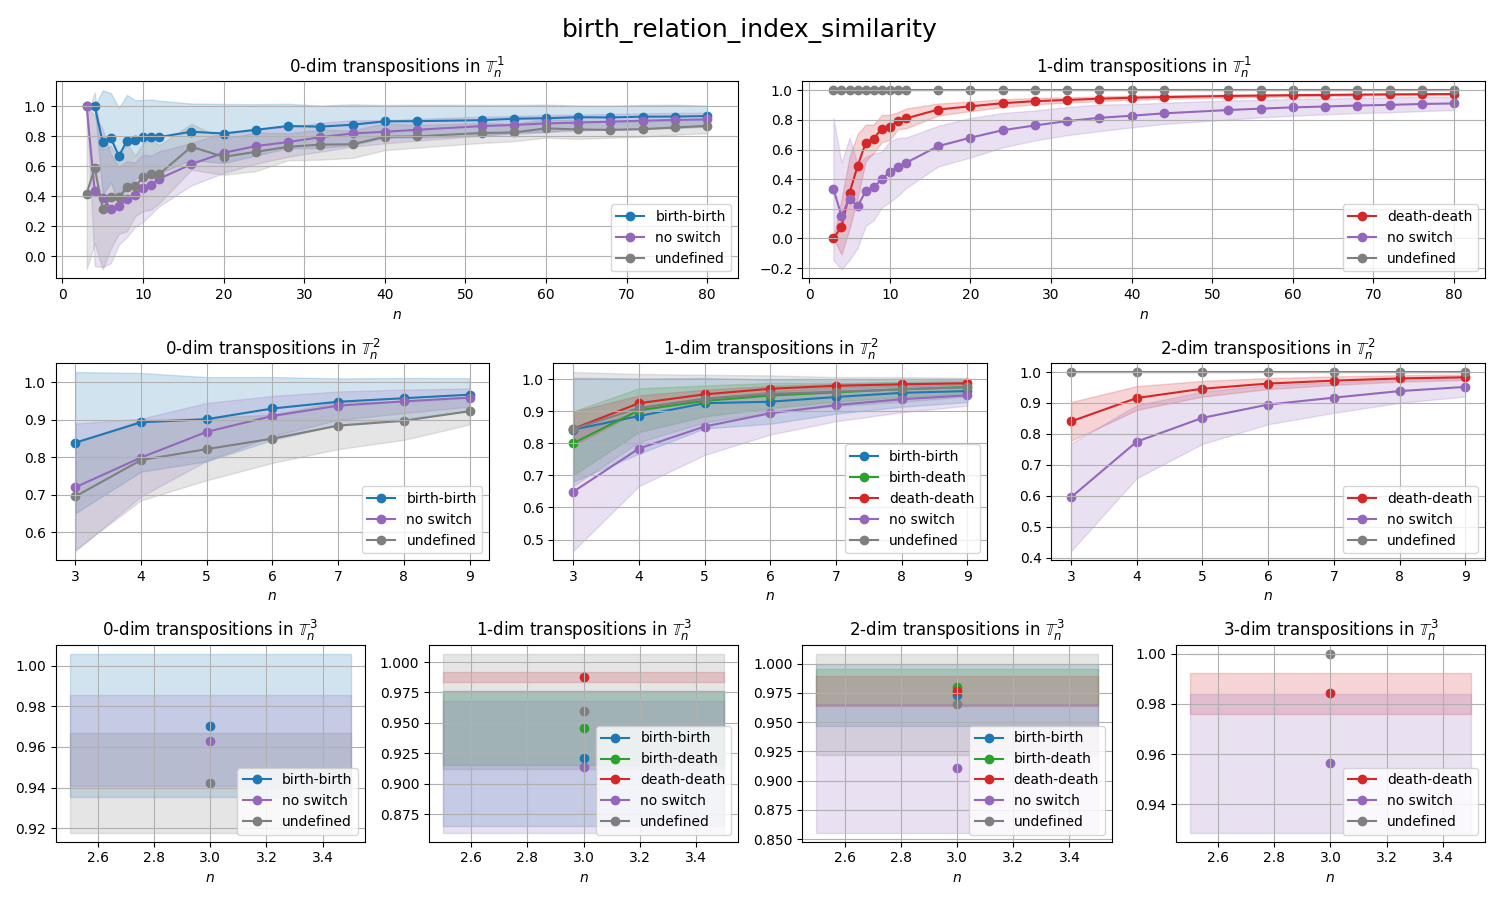
\includegraphics[width=1.5\textwidth]{pics/torus-transpositions/similaritites/score=birth-relation-index-similarity.png}
    \caption{birth\_relation\_index\_similarity values}
    \label{fig:birth-relation-index-similarity}
\end{figure}
\begin{figure}[h!]
    \hspace*{-3cm}
    \centering
    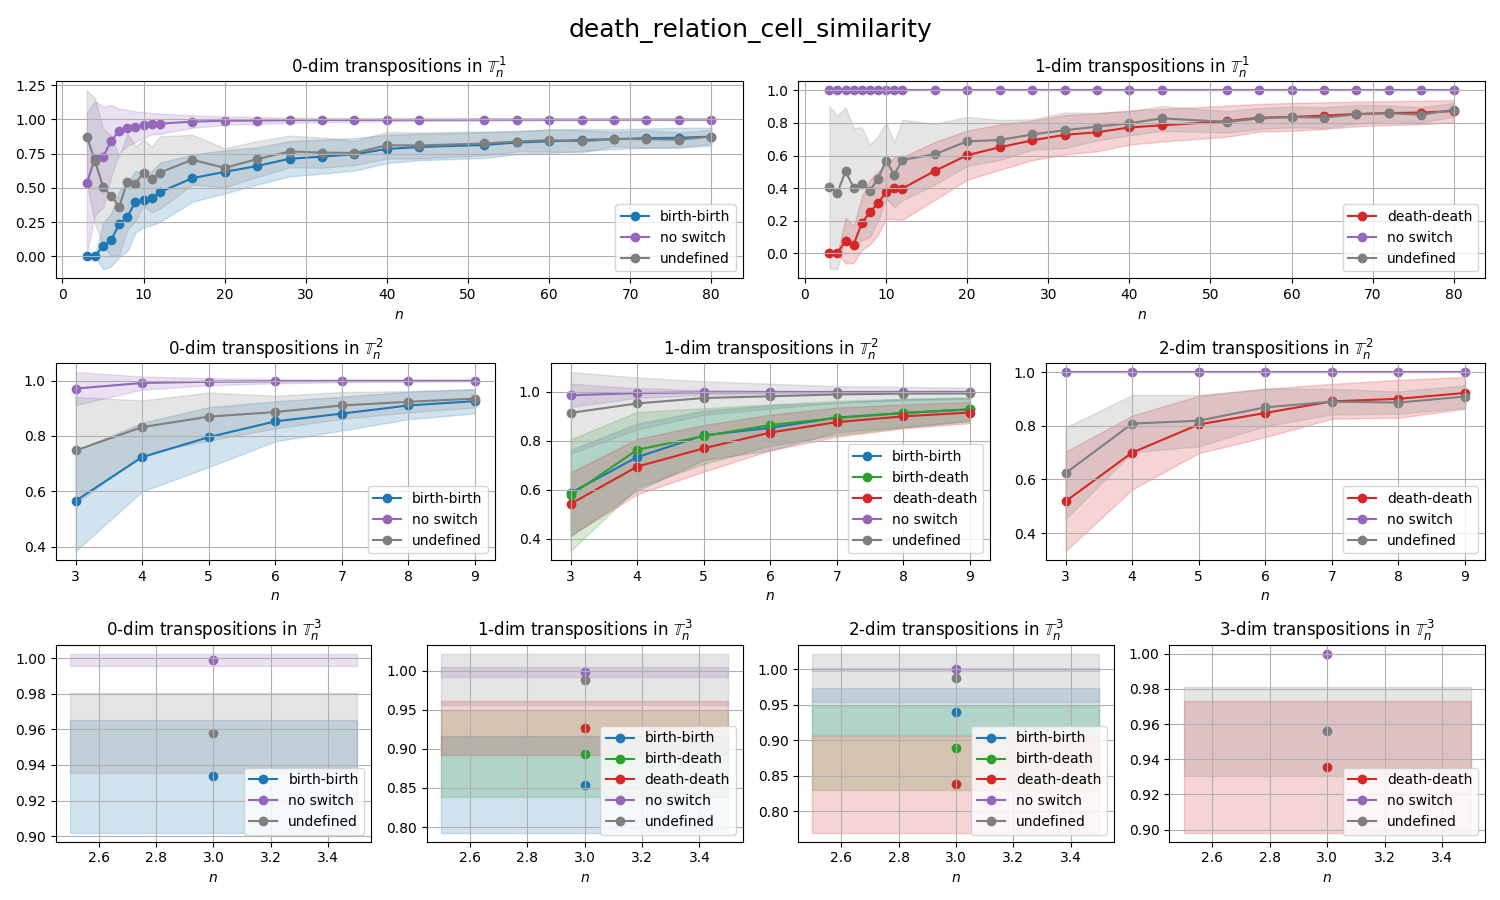
\includegraphics[width=1.5\textwidth]{pics/torus-transpositions/similaritites/score=death-relation-cell-similarity.png}
    \caption{death\_relation\_cell\_similarity values}
    \label{fig:death-relation-cell-similarity}
\end{figure}
\begin{figure}[h!]
    \hspace*{-3cm}
    \centering
    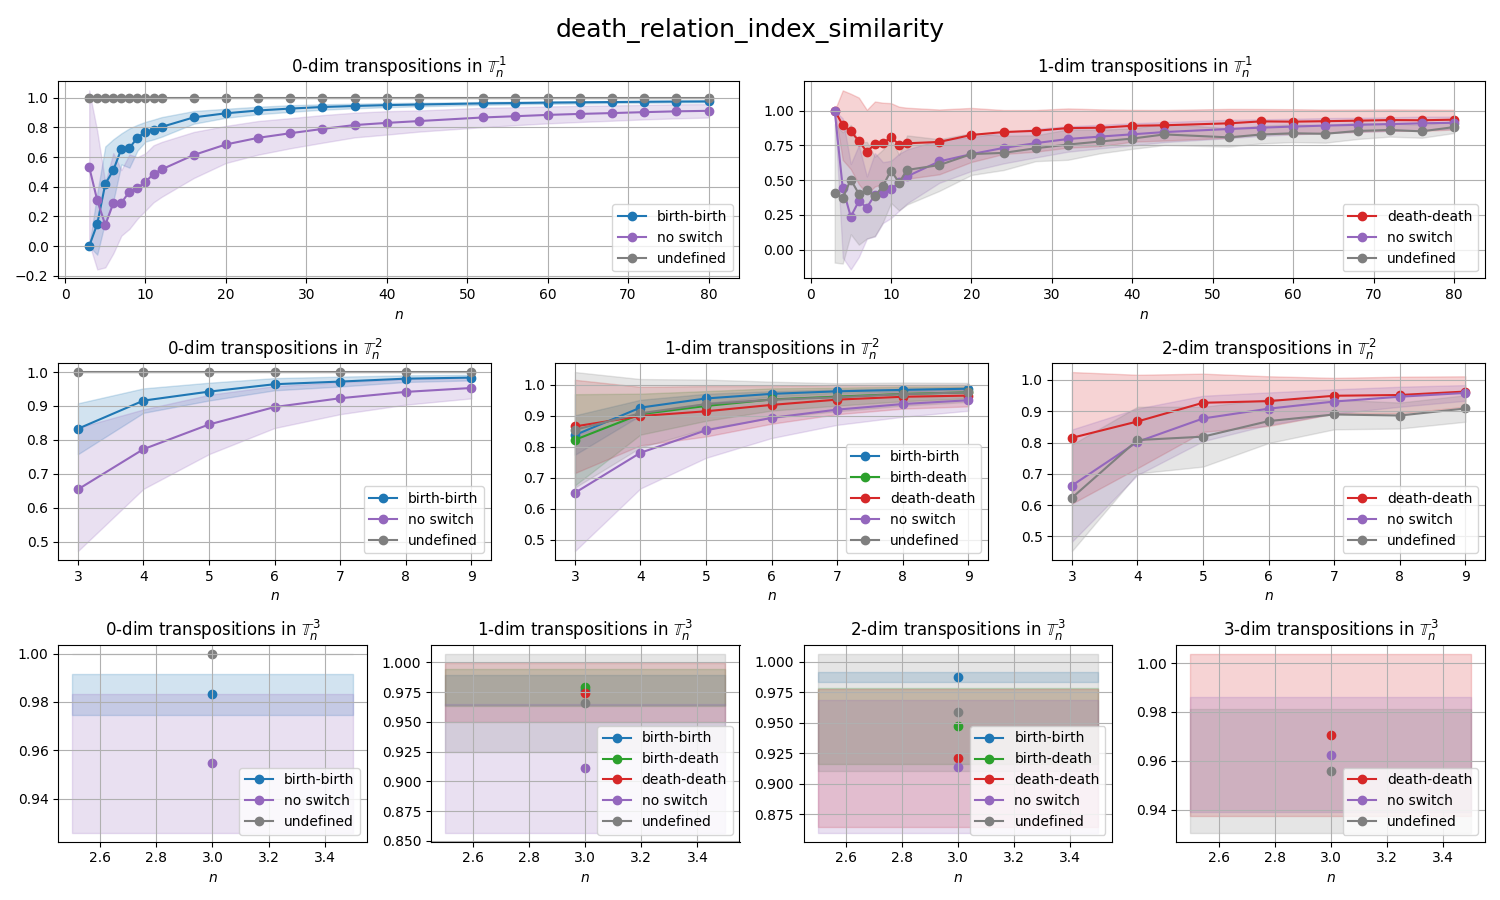
\includegraphics[width=1.5\textwidth]{pics/torus-transpositions/similaritites/score=death-relation-index-similarity.png}
    \caption{death\_relation\_index\_similarity values}
    \label{fig:death-relation-index-similarity}
\end{figure}
\begin{figure}[h!]
    \hspace*{-3cm}
    \centering
    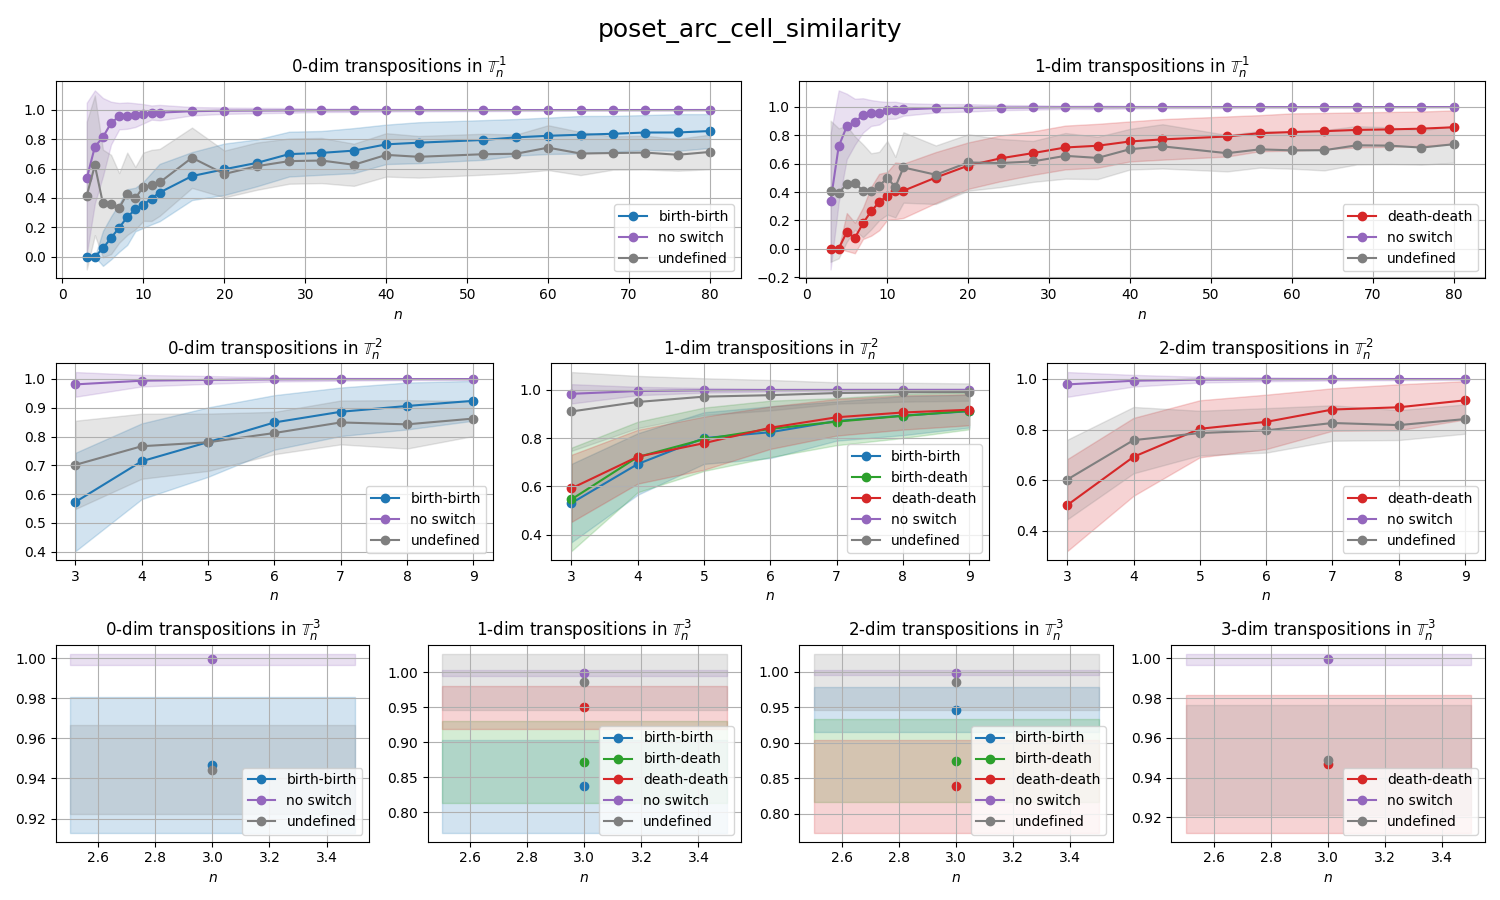
\includegraphics[width=1.5\textwidth]{pics/torus-transpositions/similaritites/score=poset-arc-cell-similarity.png}
    \caption{poset\_arc\_cell\_similarity values}
    \label{fig:poset-arc-cell-similarity}
\end{figure}
\begin{figure}[h!]
    \hspace*{-3cm}
    \centering
    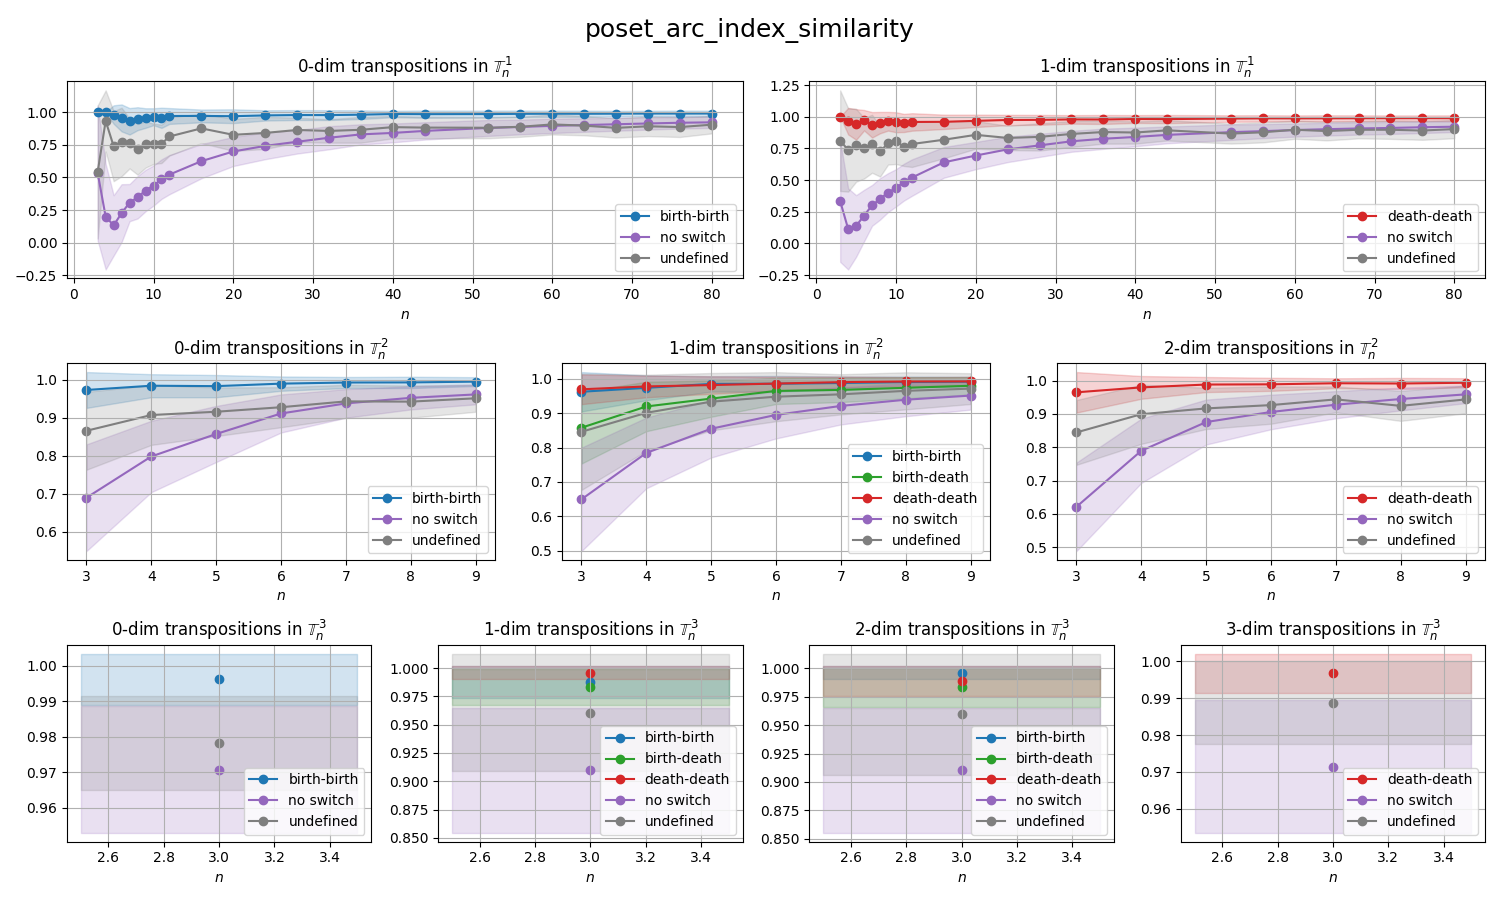
\includegraphics[width=1.5\textwidth]{pics/torus-transpositions/similaritites/score=poset-arc-index-similarity.png}
    \caption{poset\_arc\_index\_similarity values}
    \label{fig:poset-arc-index-similarity}
\end{figure}
\begin{figure}[h!]
    \hspace*{-3cm}
    \centering
    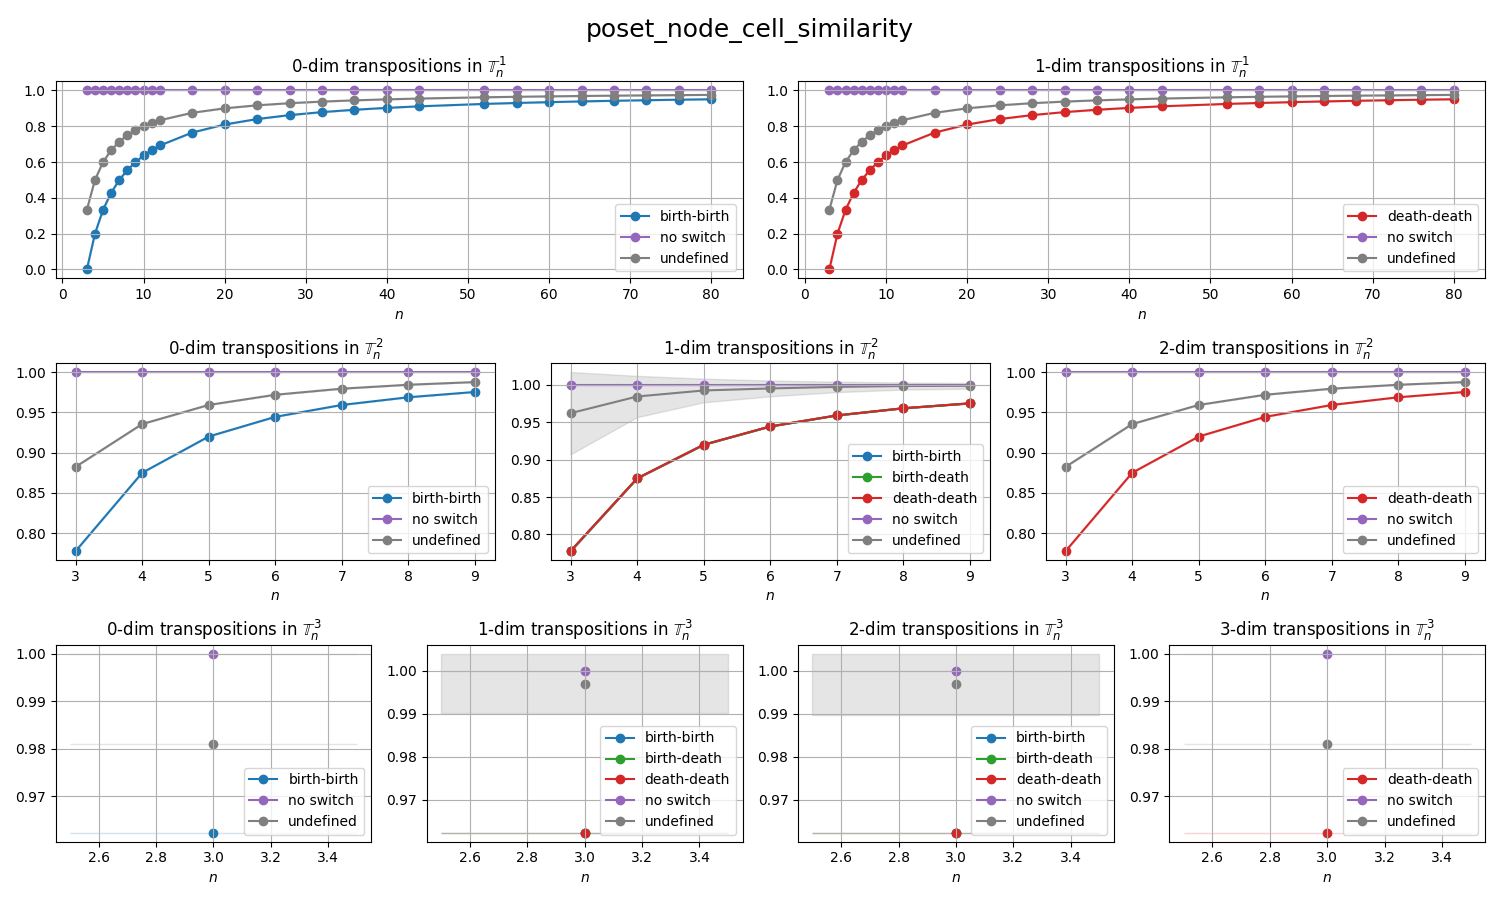
\includegraphics[width=1.5\textwidth]{pics/torus-transpositions/similaritites/score=poset-node-cell-similarity.png}
    \caption{poset\_node\_cell\_similarity values}
    \label{fig:poset-node-cell-similarity}
\end{figure}
\begin{figure}[h!]
    \hspace*{-3cm}
    \centering
    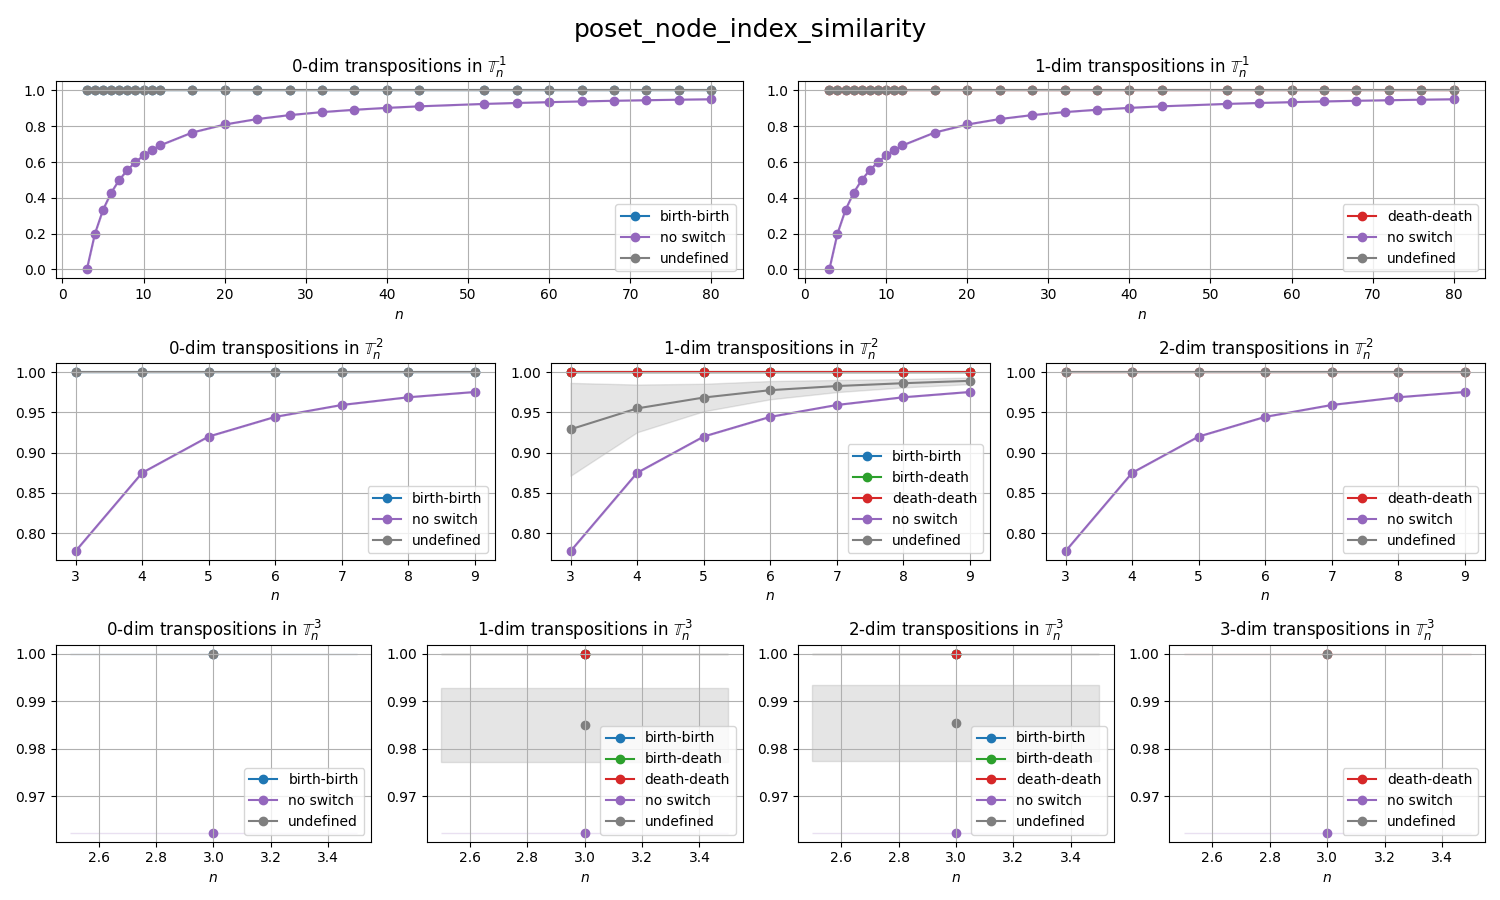
\includegraphics[width=1.5\textwidth]{pics/torus-transpositions/similaritites/score=poset-node-index-similarity.png}
    \caption{poset\_node\_index\_similarity values}
    \label{fig:poset-node-index-similarity}
\end{figure}
\begin{figure}[h!]
    \hspace*{-3cm}
    \centering
    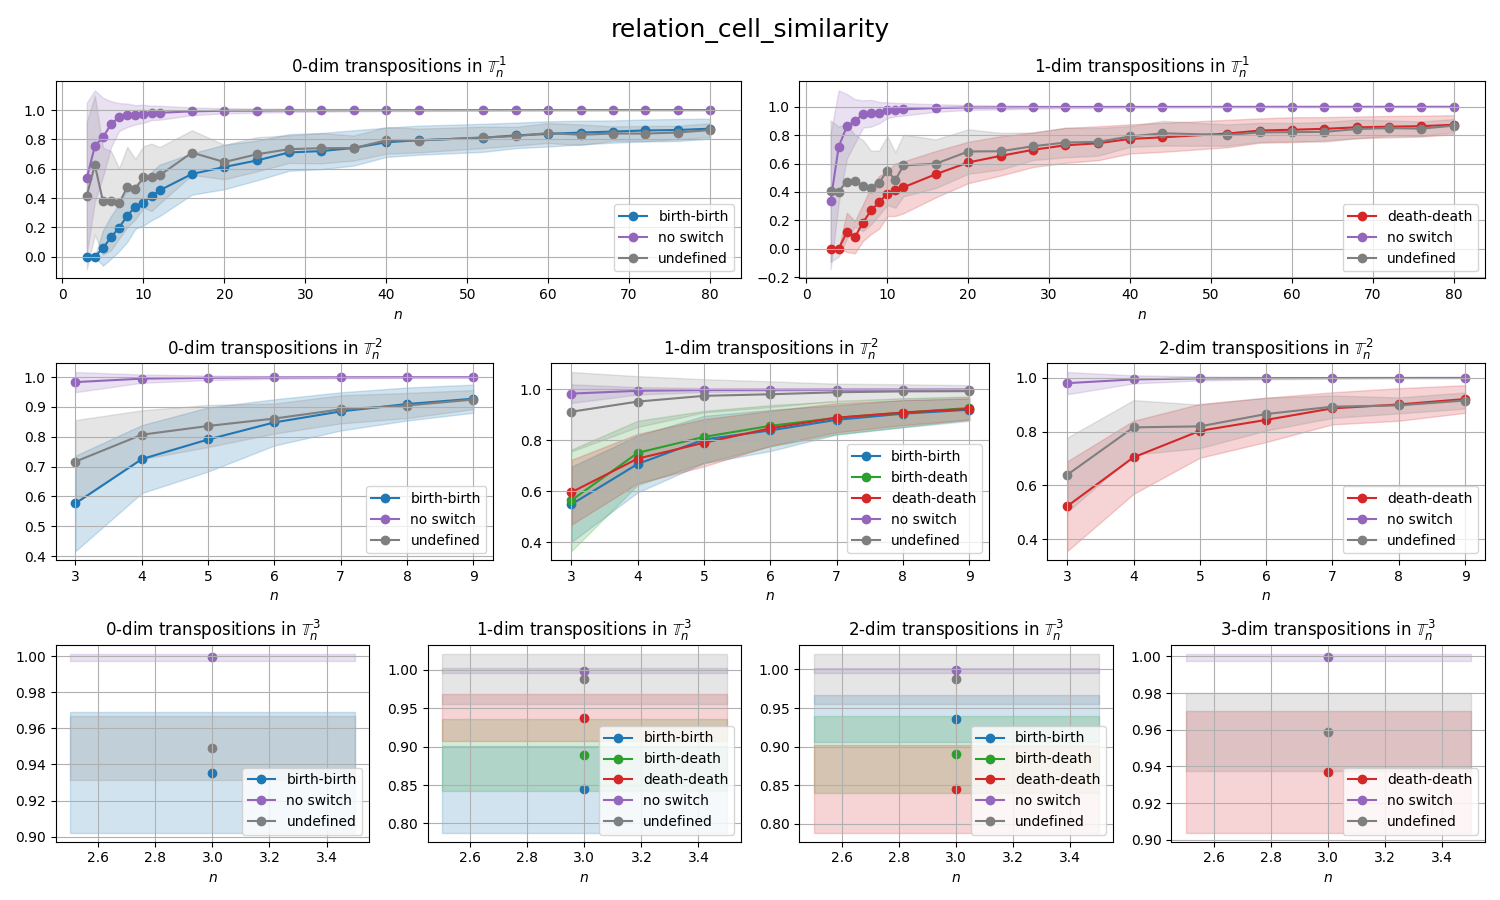
\includegraphics[width=1.5\textwidth]{pics/torus-transpositions/similaritites/score=relation-cell-similarity.png}
    \caption{relation\_cell\_similarity values}
    \label{fig:relation-cell-similarity}
\end{figure}
\begin{figure}[h!]
    \hspace*{-3cm}
    \centering
    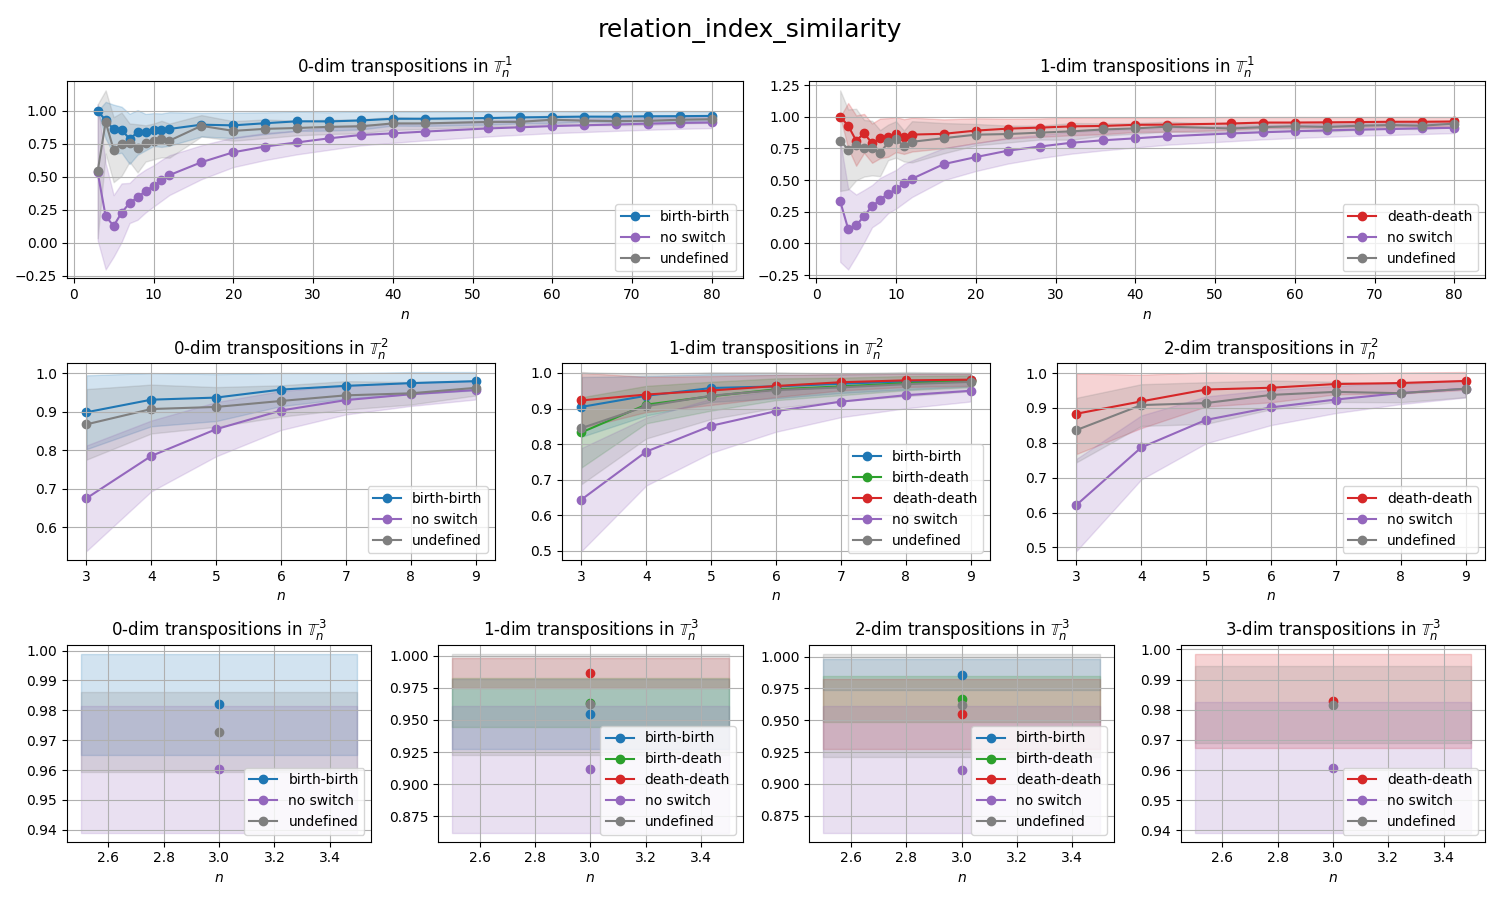
\includegraphics[width=1.5\textwidth]{pics/torus-transpositions/similaritites/score=relation-index-similarity.png}
    \caption{relation\_index\_similarity values}
    \label{fig:relation-index-similarity}
\end{figure}

\end{document}